\documentclass[letterpaper]{article}
\usepackage{aaai}
\usepackage{graphicx,curves}
\usepackage{float}
\usepackage{listings}
\title{Brachial Plexus segmentation of ultrasound by CNN}
\date{2017-11-08}
\author{David Quail\\
Department of Computing Science \\ University of Alberta \\
Edmonton, Alberta, T6G 2E8, Canada \\
dquail@ualberta.ca}
\begin{document}
\maketitle
\begin{abstract}
Pain management through the use of indwelling catheters that block or mitigate pain source, is a promising alternative to narcotics, which bring on a bevy of unwanted side effects. Accurate identification of nerve structures in ultrasound images is a fundamental step in effectively inserting a catheter into a patient requiring pain management. In this paper, we look into several different convolutional neural networks and compare their ability to segment the brachial plexus from an ultrasound image of a patient. 
\end{abstract}
    
\section{Background}

Pain control post surgery is a priority for health care providers. In addition to keeping the patient comfortable, pain management has other benefits. Pain control can help speed recover and may reduce the risk of developing certain complications after surgery, including blood clots and pneumonia. This is because, if pain is controlled, patients will be more able to complete tasks such as walking and deep breathing exercises.

The most common treatment of pain is the administration of narcotics. But these narcotics have a significant downside. These side effects include nausea, itching, and drowsiness. 

A promising alternative to pain control is creating a nerve block. Unlike an epidural which controls pain over a large region of your body, a nerve block controls pain in a smaller region of the body, such as a limb. The nerve block is created by placing thin catheter The main advantage of these nerve blocks is that they avoid the side effects common to narcotics stated above.

Creating a nerve block is done by using a needle to place a small catheter in the appropriate nerve. The main challenge in doing so is isolating the appropriate insertion place. Current methods involve using an ultrasound in real time to identify a nerve structure such as the brachial plexus. This requires the knowledge of a highly trained radiologist, and even then, is error prone. For these reasons, a less manual, and more accurate approach is desired. 

 \begin{figure}[H]
  \centerline{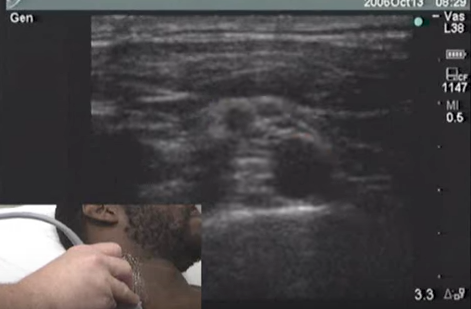
\includegraphics[width=0.5\textwidth]{Images/UltrasoundNerve.png}}
  \caption{A patient receiving an ultrasound in an effort to identify the brachial plexus. An expert radiologist could identify the nerve in the image, but it requires years of advanced training.}
  \label{fig:cnnarchitecture}
\end{figure}

A convolutional neural network (CNN) is a class of deep, feed forward artificial neural network that has been used successfully for analyzing visual imagery. They are inspired by biological processes represented within the visual cortex and in recent years, have demonstrated promise in medical image segmentation. 

These networks are known to be shift and space invariant and can learn filters that were hand engineered in traditional algorithms. This independence from prior knowledge and human effort in feature design makes them an excellent makes them an excellent candidate for an approach to automatic segmentation of nerves in ultrasound images. 



 \begin{figure}[H]
  \centerline{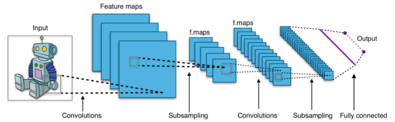
\includegraphics[width=0.5\textwidth]{Images/TypicalCNN.png}}
  \caption{Typical CNN Architecture.}
  \label{fig:cnnarchitecture}
\end{figure}

In this paper, we explore using a convolutional neural networks (CNN) to segment these ultrasound images. A UNET structure is considered the strongest for medical images because it applies a fully connected convolutional network architecture in a way the most use out of limited data, We will tune parameters within the UNET and compare its  performance to a simple Segnet structure 

\section{Experimental Setup}
For the task of segmenting MRI data using our convolution neural network, we needed to consider the training data, as well as the network infrastructure for training and prediction.

\subsection{The data}
A Kaggle competition in 2016 made available a large training set of images where the Brachial Plexus (BP) nerve has been manually annotated in ultrasound images. The annotators were trained by experts and instructed to annotate images where they were confident about the existence of the BP landmark.. This data set inckudes images where the BP is not present, and as with any human-labeled data, will ocntain noise, artifacts, and potential mistakes from the ground truth. 

 \begin{figure}[H]
  \centerline{
\includegraphics[width=0.5\textwidth]{Images/Keras.png}}
  \caption{An ultrasound image which includes the unlabelled BP.}
  \label{fig:BPInUltrasound}
\end{figure}

 \begin{figure}[H]
  \centerline{
\includegraphics[width=0.5\textwidth]{Images/Keras.png}}
  \caption{The human labelled mask for the ultrasound of the BP.}
  \label{fig:BPMask}
\end{figure}

\subsection{CNN Implementation libraries}
In order to build the different convolutional neural networks used to segment the ultrasound images, we wanted to use a high-level neural network API that enabled fast experimentation. The Keras API library is one such solution, and the one we chose. Keras is written in Python and is capable of running on top of TensorFlow - an open source software library for numerical computation using data flow graphs. Keras and TensorFlow support both convolutional networks and runs seamlessly on CPU and GPU. 

 \begin{figure}[H]
  \centerline{
\includegraphics[width=0.5\textwidth]{Images/Keras.png}}
  \caption{Keras.}
  \label{fig:keras}
\end{figure}

Experiments were run using an amazon EC2 instance with a GPU using cuDNN - a deep neural network GPU accelerated library. This approach is much faster than a typical CPU because of the parallel computation it was designed form,

\section{2 Dimensional UNET CNN}

\subsection{Network design}
The U-Net is a network design that relies on strong use of data augmentation to use the available annotated samples more efficiently. The architecture contains a contracting path which captures context and a symmetric expanding path that enables precise localization. It is called a "U-net" because of it's "U" shaped network structure.


 \begin{figure}[H]
  \centerline{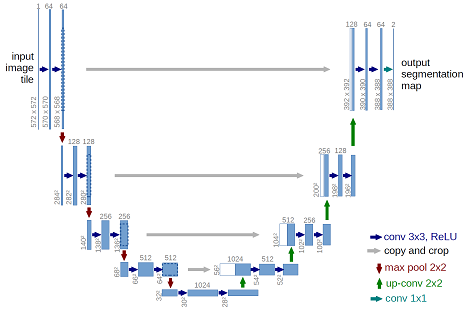
\includegraphics[width=0.5\textwidth]{Images/UNET.png}}
  \caption{U-Net architecture.}
  \label{fig:unet}
\end{figure}

As seen above, the U-Net network takes a raw image as input and outputs an output segmentation map. 
It's overall architecture is illustrated below. Like any convolutional neural network, it consists of a number of small operations, each of which corresponding to a small arrow below. The image file is input into the network and the propogated through the network along all possible paths,  and at the end, the ready segmentation map is output.

Each blue box corresponds to a multi channel feature layer. Most of the operations are convolutions followed by a non-linear feature activation. 

Below is a diagram detailing one of the first convolution layer. The layer contains of the standard 3X3 convolution followed by a non-linear activation function. By design, only the valid part of the convolution is used, which means that for a 3X3 convolution, a 1 pixel border is lost. This allows large images to be processed in smaller tiles. 	

 \begin{figure}[H]
  \centerline{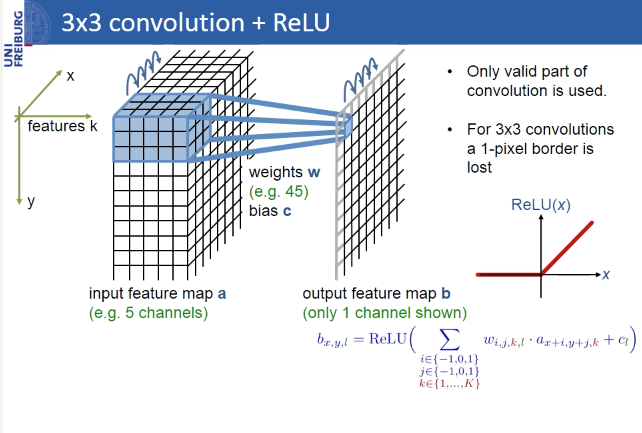
\includegraphics[width=0.5\textwidth]{Images/UNET1.png}}
  \caption{Convolution layer.}
  \label{fig:unet1}
\end{figure}

Max pooling operations as seen below are illustrated with down arrows in the architecture diagram. It reduces the x, y size of the feature map. This max pooling operation operates on each channel separately.  This simply propogates the maximum activation from each 2X2 window to the next feature map. After each max pooling operation, the number of feature channels are increased by a factor of 2. All in all, these convolution and pooling operations gradually increase the "what" and decrease the "where." In other words, it is able to identify shift and space invariant features. 


 \begin{figure}[H]
  \centerline{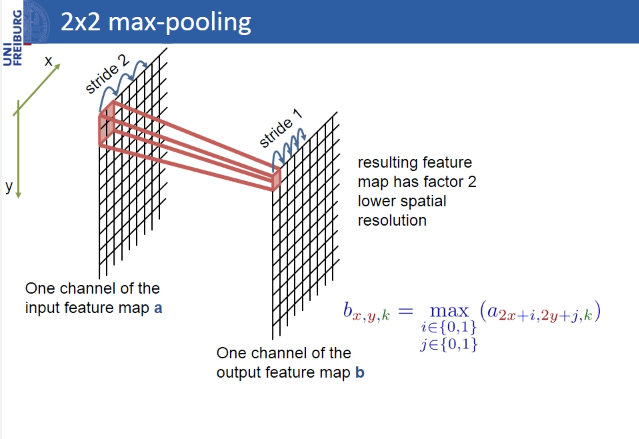
\includegraphics[width=0.5\textwidth]{Images/UNET2.png}}
  \caption{2X2 max pooling.}
  \label{fig:unet2}
\end{figure}

Finally, after these contraction operations, expansion operations are performed to create a high segmentation map of the same resolution as the original image.  	

 \begin{figure}[H]
  \centerline{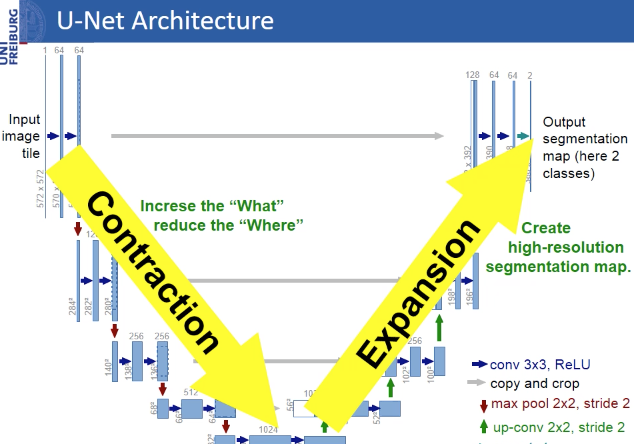
\includegraphics[width=0.5\textwidth]{Images/UNET3.png}}
  \caption{Expansion of the image}
  \label{fig:unet3}
\end{figure}


The following is the Python code used to create the UNET. 

 \begin{figure}[H]
  \centerline{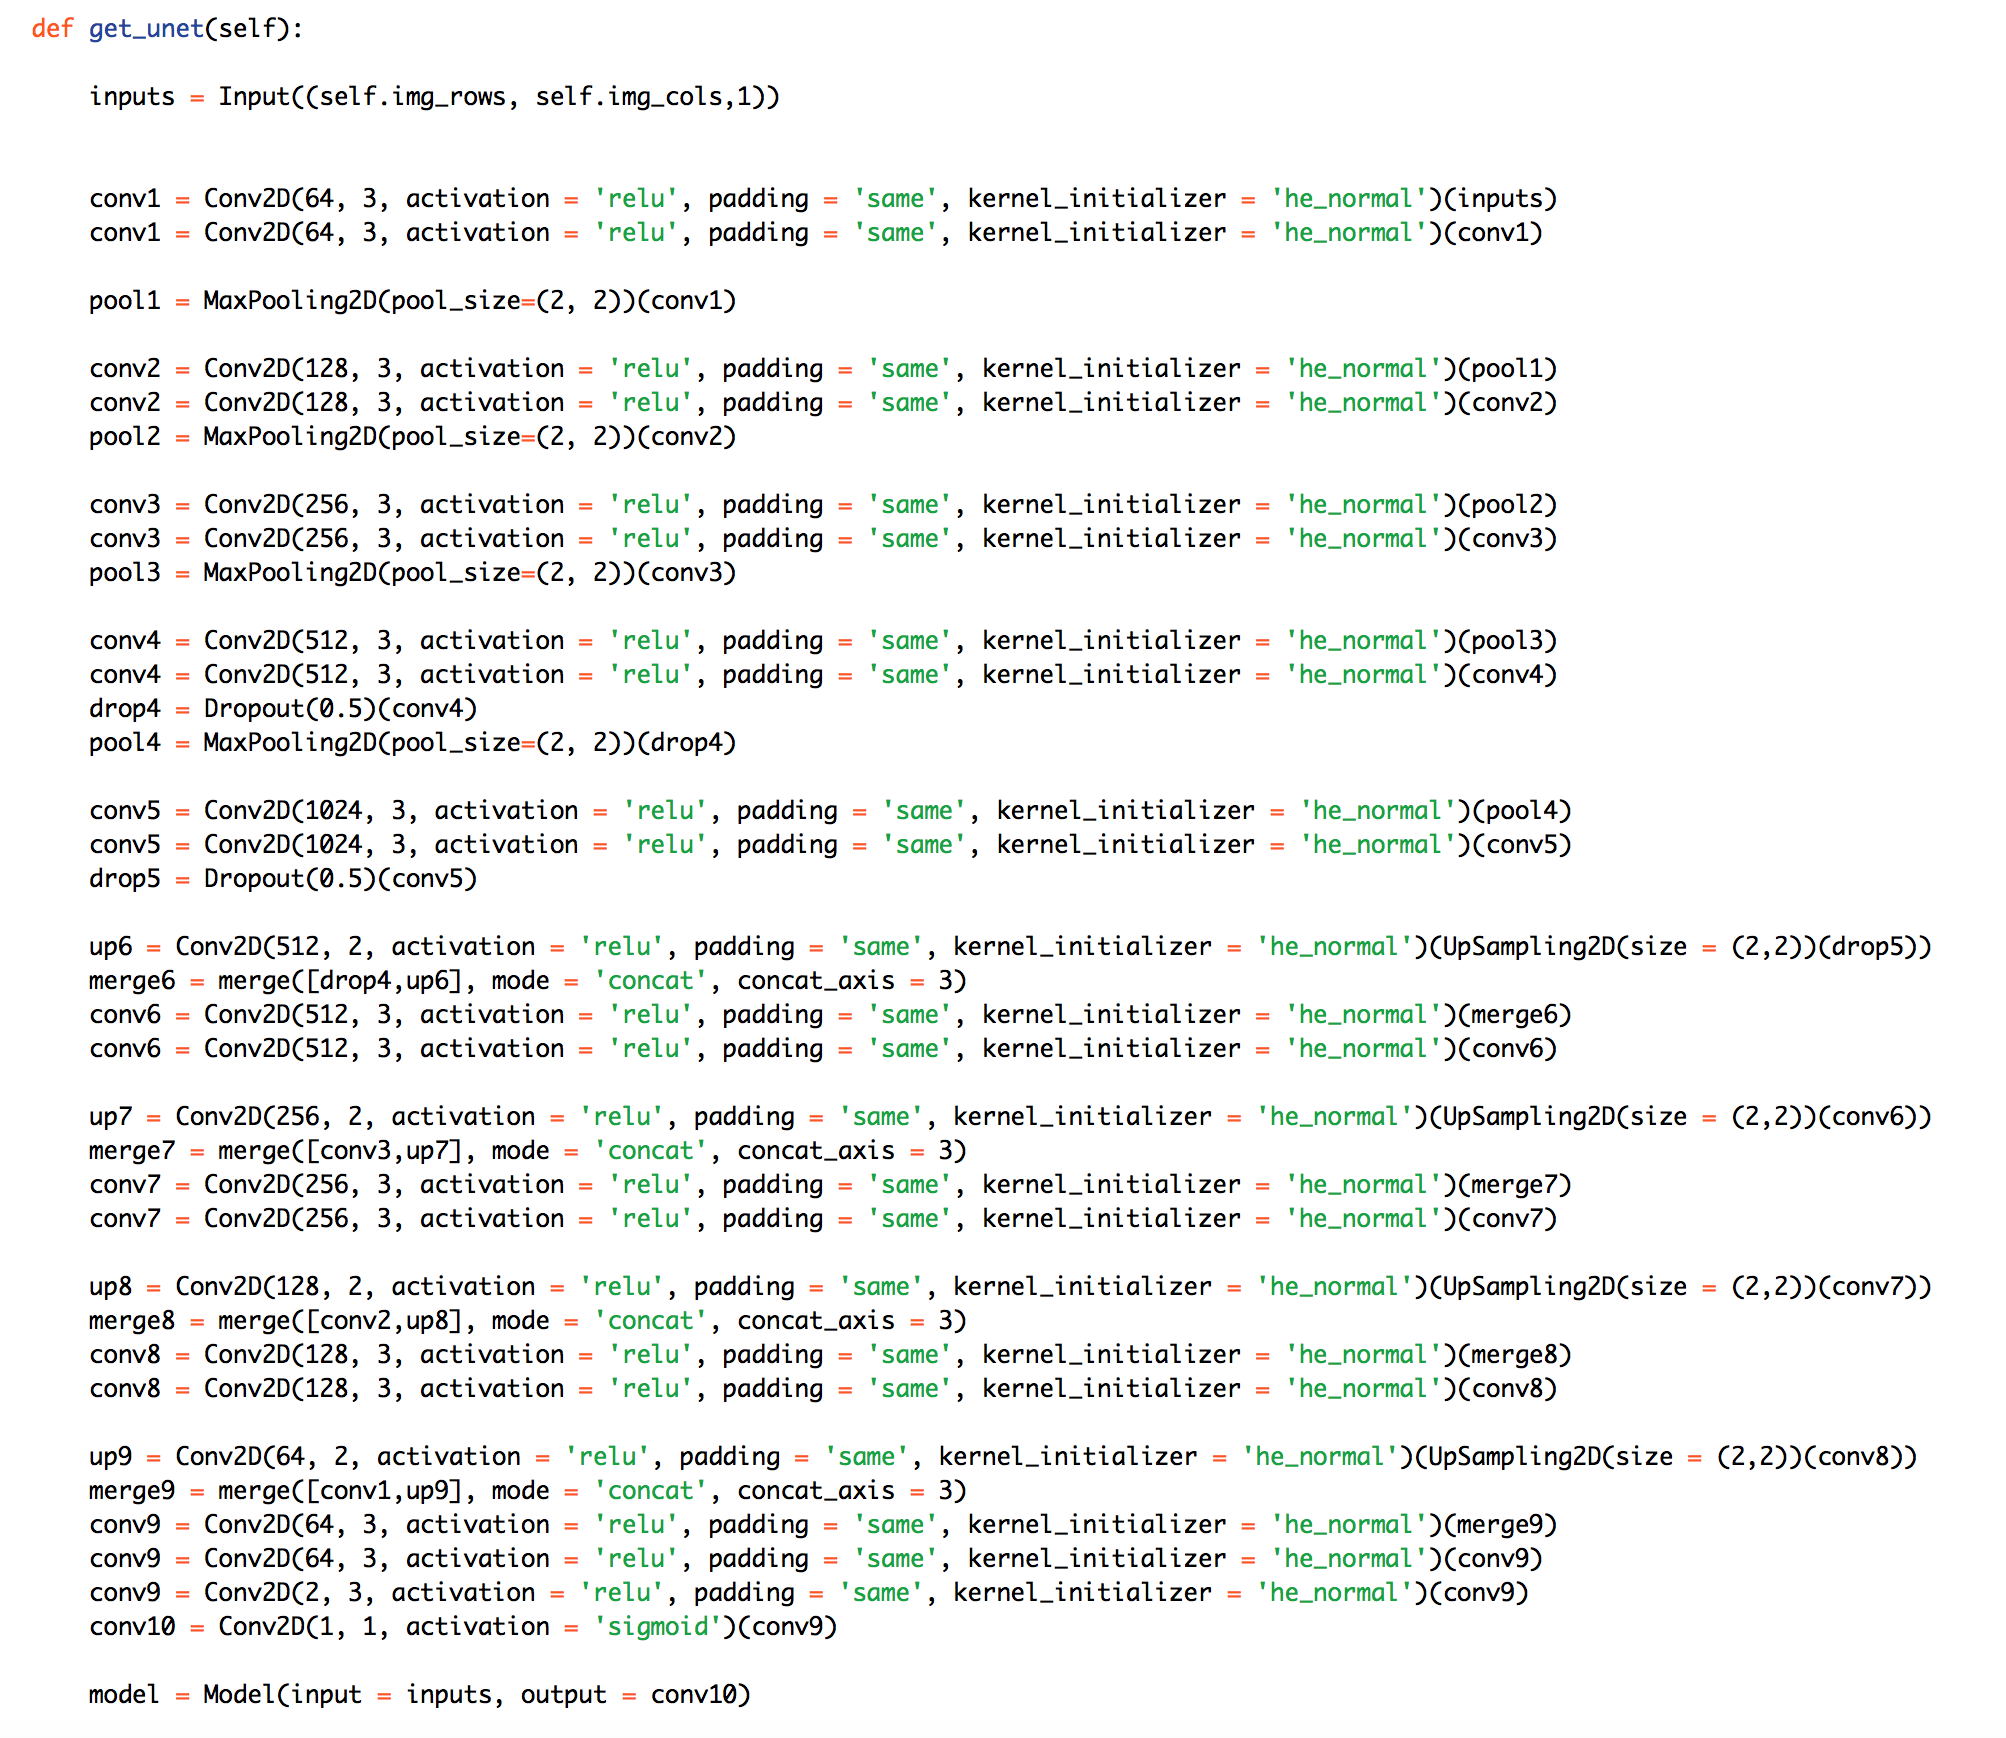
\includegraphics[width=0.5\textwidth]{Images/KerasUNET.png}}
  \caption{Creating the UNET using keras and tensorflow.}
  \label{fig:kerasunet3}
\end{figure}

A dice coeficcient loss function is used. 

$$\sum_{i=1} H(yi', yi)$$

 \begin{figure}[H]
  \centerline{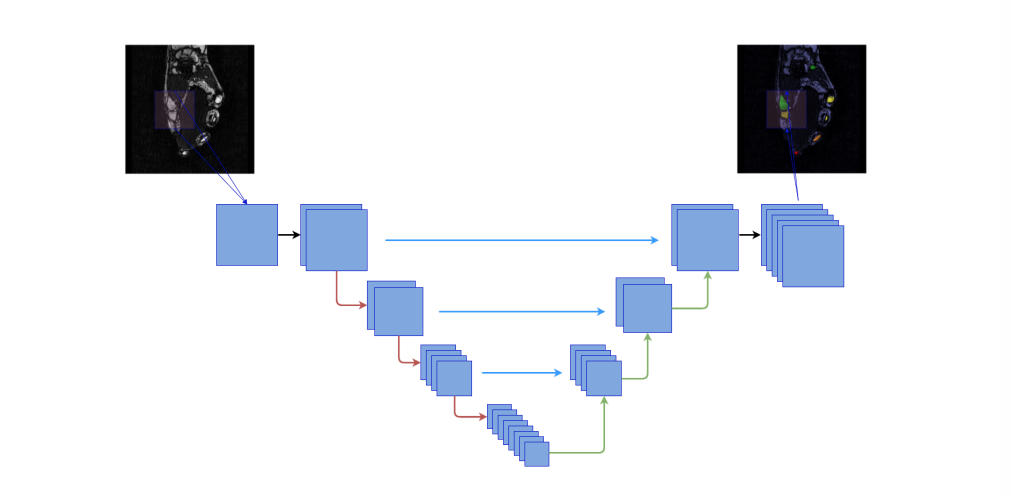
\includegraphics[width=0.5\textwidth]{Images/UNETMedical.png}}
  \caption{A U-Net architecture in a more abstract form. The actual number of feature maps illustrated is symbolic. The green arrows do unsampling and black ones keep the original size of input, while arrows marked red are blocks of layers that downsample their input. The cyan arrows are long skip connections which concatenate feature maps from the first stage to feature maps in the second stage. This results in the expanding path having access to twice as many features as the contracting path.}
  \label{fig:kerasunet3}
\end{figure}


\subsection{Data augmentation}
The training data available for our task, therefore, we use excessive data augmentation by applying elastic deformations to the training images. This allows the network to learn invariance to deformations without seeing them in the segmentation training data. In biomedical segmentation, this is important, since deformation used to be the most common variation in tissue and these deformations can be simulated efficiently. 

 \begin{figure}[H]
  \centerline{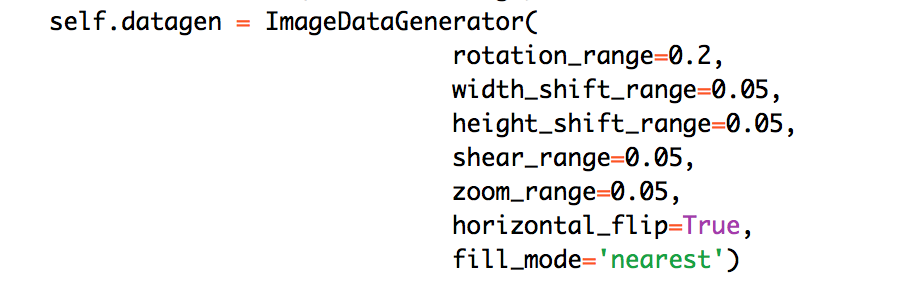
\includegraphics[width=0.5\textwidth]{Images/KerasDataAugmentation.png}}
  \caption{Augmenting the image data using keras data augmentation abilities.}
  \label{fig:unet3}
\end{figure}

The descriptions for the augmentation variables are as follows:

\begin{itemize}
  \item rotation\_range = Degree range for random rotations.
  \item width\_shift\_range =  Range for random horizontal shifts. (fraction of total width). 
  \item height\_shift\_range = Range for random vertical shifts. (fraction of total height)
  \item shear\_range = Shear Intensity (Shear angle in counter-clockwise direction as radians)
  \item zoom\_range = Range for random zoom.
\end{itemize}



\subsection{Results}
The training examples were randomly split. 80 percent were reserved for training, and the remaining 20 percent for testing the performance of the resulting model.

A mask is created for each test example as seen below.

 \begin{figure}[H]
  \centerline{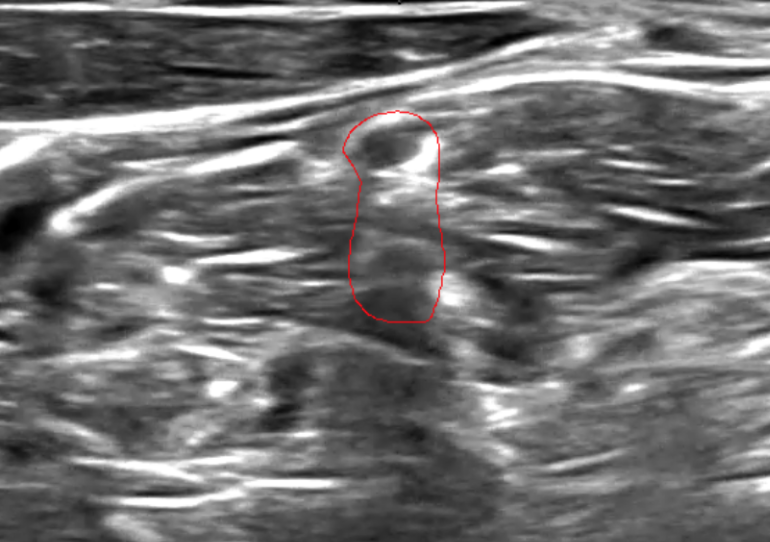
\includegraphics[width=0.5\textwidth]{Images/SegmentExample1.png}}
  \caption{An example of a resulting image segmentation. For the purposes of illustration, the area inside the red circle is the area that has been segmented as the BP}
  \label{fig:BPSegmentation1}
\end{figure}

 \begin{figure}[H]
  \centerline{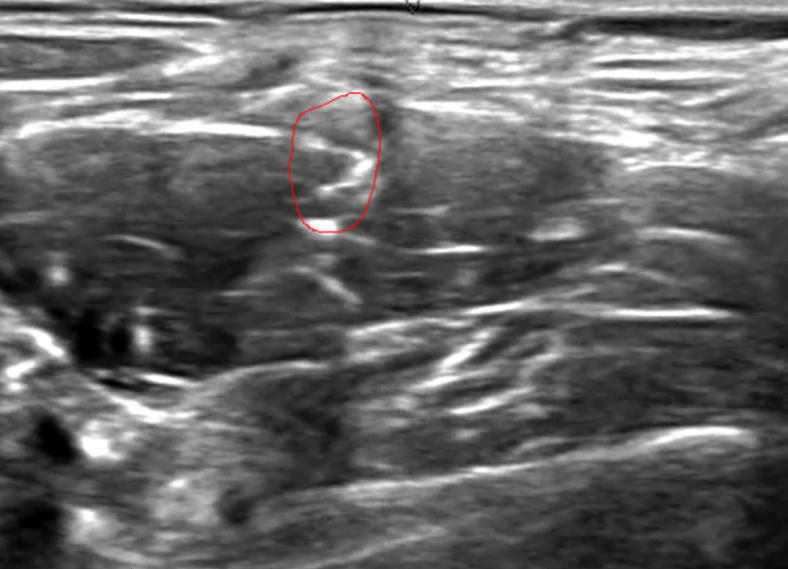
\includegraphics[width=0.5\textwidth]{Images/SegmentExample2.png}}
  \caption{A second example of the BP segmentation.}
  \label{fig:BPSegmentation2}
\end{figure}

 \begin{figure}[H]
  \centerline{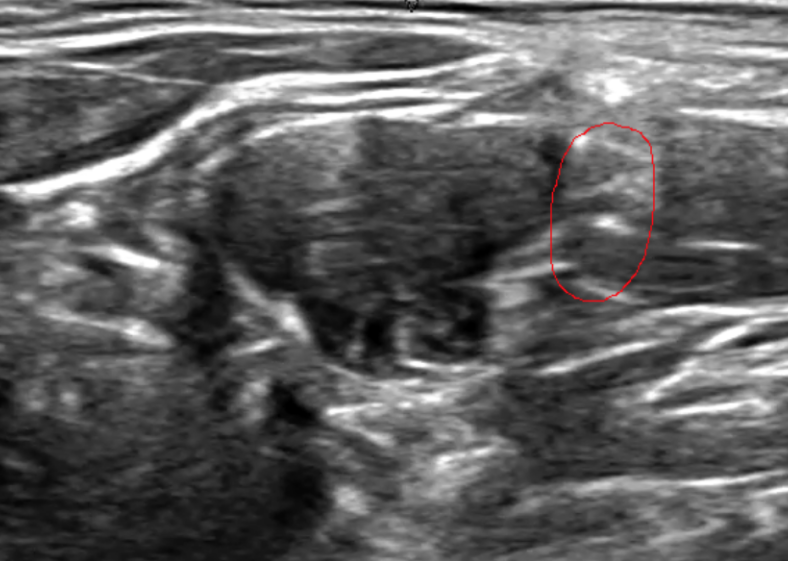
\includegraphics[width=0.5\textwidth]{Images/SegmentExample3.png}}
  \caption{A third example of a BP segmentation}
  \label{fig:BPSegmentation3}
\end{figure}

The resulting dice coefficient (DCF) is used for a performance measure as well as the loss function. 

A DCF of 0.65 is achieved with a simple UNET architecture after 20 epochs of training with batch sizes of 32. 

 \begin{figure}[H]
  \centerline{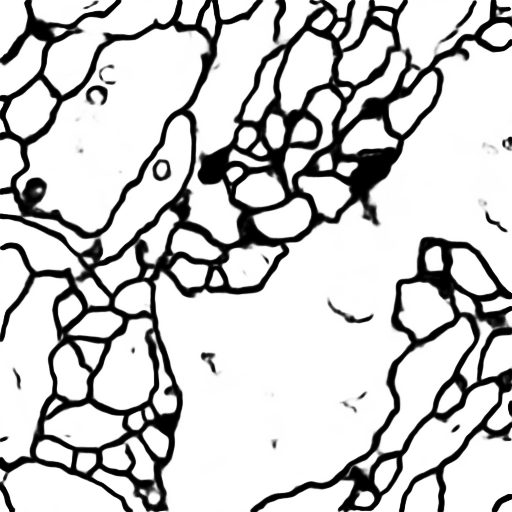
\includegraphics[width=0.5\textwidth]{Images/MRISegment.png}}
  \caption{The resulting image segmentation after training}
  \label{fig:mrisegment}
\end{figure}

\section{Conclusions}
This seems to be a promising approach for segmentation.
\section{Future work}
There are a number of different network configurations that could be considered. 
\begin{itemize}
  \item More than just UNET 
\end{itemize}
\bibliographystyle{aaai}
\bibliography{bibliography}
\end{document}